
\documentclass{article}

\usepackage{amsmath,amsfonts,stmaryrd,amssymb} % Math packages

\usepackage{enumerate} % Custom item numbers for enumerations

\usepackage[ruled]{algorithm2e} % Algorithms

\usepackage[framemethod=tikz]{mdframed} % Allows defining custom boxed/framed environments

\usepackage{listings} % File listings, with syntax highlighting
\lstset{
	basicstyle=\ttfamily, % Typeset listings in monospace font
}

\usepackage{amsmath,amsfonts,stmaryrd,amssymb} 
\usepackage{enumerate} 
\usepackage[ruled]{algorithm2e} 
\usepackage[framemethod=tikz]{mdframed}
\usepackage{listings} 
\lstset{
	basicstyle=\ttfamily, 
}
\usepackage{geometry} 
\geometry{
	paper=a4paper, % Paper size, change to letterpaper for US letter size
	top=2cm, % Top margin
	bottom=1cm, % Bottom margin
	left=2.5cm, % Left margin
	right=2.5cm, % Right margin
	headheight=14pt, % Header height
	footskip=1.5cm, % Space from the bottom margin to the baseline of the footer
	headsep=1.2cm, % Space from the top margin to the baseline of the header
	%showframe, % Uncomment to show how the type block is set on the page
}

\usepackage[utf8]{inputenc} % Required for inputting international characters
\usepackage[T1]{fontenc} % Output font encoding for international characters

\usepackage{XCharter} % Use the XCharter fonts

%----------------------------------------------------------------------------------------
%	COMMAND LINE ENVIRONMENT
%----------------------------------------------------------------------------------------

% Usage:
% \begin{commandline}
%	\begin{verbatim}
%		$ ls
%		
%		Applications	Desktop	...
%	\end{verbatim}
% \end{commandline}

\mdfdefinestyle{commandline}{
	leftmargin=10pt,
	rightmargin=10pt,
	innerleftmargin=15pt,
	middlelinecolor=black!50!white,
	middlelinewidth=2pt,
	frametitlerule=false,
	backgroundcolor=black!5!white,
	frametitle={Command Line},
	frametitlefont={\normalfont\sffamily\color{white}\hspace{-1em}},
	frametitlebackgroundcolor=black!50!white,
	nobreak,
}

% Define a custom environment for command-line snapshots
\newenvironment{commandline}{
	\medskip
	\begin{mdframed}[style=commandline]
}{
	\end{mdframed}
	\medskip
}
% Usage:
% \begin{file}[optional filename, defaults to "File"]
%	File contents, for example, with a listings environment
% \end{file}

\mdfdefinestyle{file}{
	innertopmargin=1.6\baselineskip,
	innerbottommargin=0.8\baselineskip,
	topline=false, bottomline=false,
	leftline=false, rightline=false,
	leftmargin=0.5cm,
	rightmargin=0.5cm,
	singleextra={%
		\draw[fill=black!10!white](P)++(0,-1.2em)rectangle(P-|O);
		\node[anchor=north west]
		at(P-|O){\ttfamily\mdfilename};
		%
		\def\l{3em}
		\draw(O-|P)++(-\l,0)--++(\l,\l)--(P)--(P-|O)--(O)--cycle;
		\draw(O-|P)++(-\l,0)--++(0,\l)--++(\l,0);
	},
	nobreak,
}

% Define a custom environment for file contents
\newenvironment{file}[1][File]{ % Set the default filename to "File"
	\medskip
	\newcommand{\mdfilename}{#1}
	\begin{mdframed}[style=file]
}{
	\end{mdframed}
	\medskip
}

%----------------------------------------------------------------------------------------
%	NUMBERED QUESTIONS ENVIRONMENT
%----------------------------------------------------------------------------------------

% Usage:
% \begin{question}[optional title]
%	Question contents
% \end{question}

\mdfdefinestyle{question}{
	innertopmargin=1.2\baselineskip,
	innerbottommargin=0.8\baselineskip,
	roundcorner=5pt,
	nobreak,
	singleextra={%
		\draw(P-|O)node[xshift=1em,anchor=west,fill=white,draw,rounded corners=5pt]{%
		Question \theQuestion\questionTitle};
	},
}

\newcounter{Question} % Stores the current question number that gets iterated with each new question

% Define a custom environment for numbered questions
\newenvironment{question}[1][\unskip]{
	\bigskip
	\stepcounter{Question}
	\newcommand{\questionTitle}{~#1}
	\begin{mdframed}[style=question]
}{
	\end{mdframed}
	\medskip
}

\mdfdefinestyle{warning}{
	topline=false, bottomline=false,
	leftline=false, rightline=false,
	nobreak,
	singleextra={%
		\draw(P-|O)++(-0.5em,0)node(tmp1){};
		\draw(P-|O)++(0.5em,0)node(tmp2){};
		\fill[black,rotate around={45:(P-|O)}](tmp1)rectangle(tmp2);
		\node at(P-|O){\color{white}\scriptsize\bf !};
		\draw[very thick](P-|O)++(0,-1em)--(O);%--(O-|P);
	}
}

% Define a custom environment for warning text
\newenvironment{warn}[1][Warning:]{ % Set the default warning to "Warning:"
	\medskip
	\begin{mdframed}[style=warning]
		\noindent{\textbf{#1}}
}{
	\end{mdframed}
}

\mdfdefinestyle{info}{%
	topline=false, bottomline=false,
	leftline=false, rightline=false,
	nobreak,
	singleextra={%
		\fill[black](P-|O)circle[radius=0.4em];
		\node at(P-|O){\color{white}\scriptsize\bf i};
		\draw[very thick](P-|O)++(0,-0.8em)--(O);%--(O-|P);
	}
}

% Define a custom environment for information
\newenvironment{info}[1][Info:]{ % Set the default title to "Info:"
	\medskip
	\begin{mdframed}[style=info]
		\noindent{\textbf{#1}}
}{
	\end{mdframed}
}
 % Include the file specifying the document structure and custom commands

%----------------------------------------------------------------------------------------
%	ASSIGNMENT INFORMATION
%----------------------------------------------------------------------------------------
\title{Operational Statistics for SAR Imagery Course Assignment} % Title of the assignment

\author{rui qi lei\\ \texttt{19171213813}} % Author name and email address

\date{Xidian University --- \today} % University, school and/or department name(s) and a date


%----------------------------------------------------------------------------------------

\begin{document}
	
	\maketitle % Print the title
	
	%----------------------------------------------------------------------------------------
	%	INTRODUCTION
	%----------------------------------------------------------------------------------------
	\section*{Urban SAR image analysis} % Unnumbered section
	\par Synthetic aperture radar is a type of microwave imaging radar. It is also an airborne or spaceborne radar that can produce high-resolution images.In its early days, it used lensing to form images on negative plates (film), and now USES sophisticated radar data post-processing to obtain extremely narrow effective radiation beams (meaning very high spatial resolution for the resulting radar image).It is usually mounted on a moving carrier to image a relatively stationary target, or vice versa.Through some assumptions and analysis, it can be found that SAR data obeys gaussian random distribution.Its intensity obeys exponential distribution.I select a sample from either urban from the image shown in Fig. 3.4,By visualizing the gray scale of the image, it can be found that its distribution is closest to that of G0.The formula for the gamma ,K and GI0 distribution is as follows:
	% Math equation/formula
	
	\begin{eqnarray}
	Gamma:f(x)=\frac{L^L}{\sigma^{2^L}\Gamma(L)}z^(L-1)exp{\lbrace{-Lz}/\sigma^2\rbrace}
	\end{eqnarray}
	
	\begin{equation}
	\mathop {K:f(x)=\frac{2\lambda L}{\Gamma(\alpha)\Gamma(L)}(\lambda Lz)^{\frac{\alpha+L}{2}-1}K_{\alpha-L}(2\sqrt{\lambda Lz})}
	\end{equation}
	\begin{equation}
	\mathop {G0:f(x)=\frac{L^L\Gamma(L-\alpha)}{\gamma^\alpha\Gamma(L)\Gamma(-\alpha)}\frac{z^{L-1}}{{(\gamma+Lz)}^{L-\alpha}}}
	\end{equation}
	\par The gamma distribution is figured below:
	\begin{figure}[h] % [h] forces the figure to be output where it is defined in the code (it suppresses floating)
		\centering
		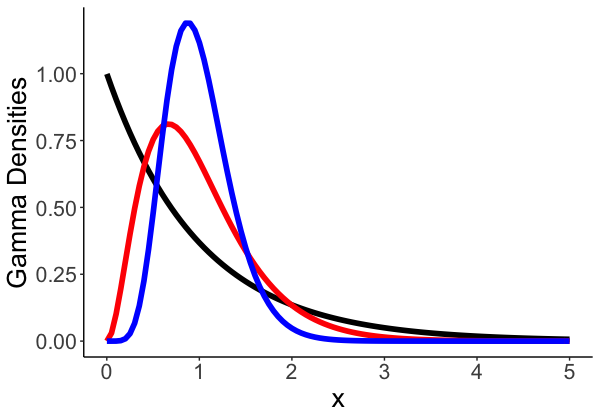
\includegraphics[width=2in]{homework/picture/gamma.png}
		\caption{Gamma distribution}
	\end{figure}
	
	\par The K distribution is figured below:
	\begin{figure}[h] % [h] forces the figure to be output where it is defined in the code (it suppresses floating)
		\centering
		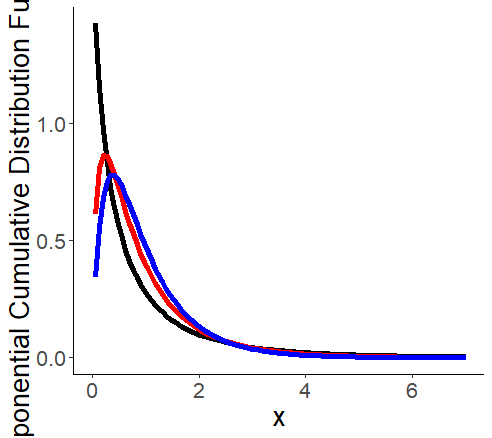
\includegraphics[width=2in]{homework/picture/K.png}
		\caption{K distribution}
	\end{figure}
	
	\par The G0 distribution is figured below:
	\begin{figure}[h] % [h] forces the figure to be output where it is defined in the code (it suppresses floating)
		\centering
		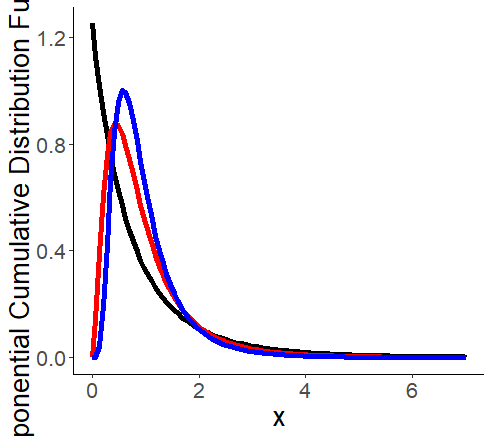
\includegraphics[width=2in]{homework/picture/g0.png}
		\caption{K distribution}
	\end{figure}
	
	\par I selected a small piece of SAR image of the city for analysis.The image below shows the original SAR image on the left and the cropped city image on the right in figure6.The original image size is829x330,and the size of the cropped image is 500x199.The gray scale of the image is analyzed, and its histogram is shown in figure 4
	
	\begin{figure}[h] % [h] forces the figure to be output where it is defined in the code (it suppresses floating)
    	\centering
    	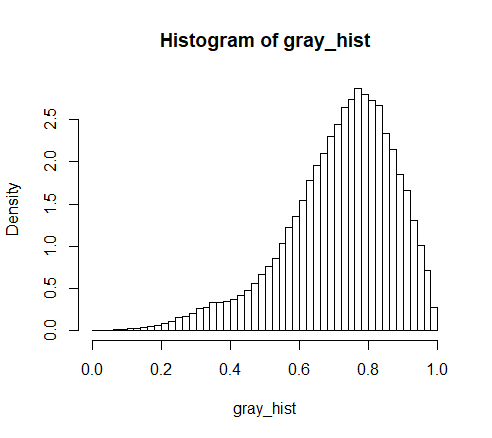
\includegraphics[width=4in]{homework/picture/gray_hist.png} 
    	\caption{ hist distribution}
    \end{figure}
	\par I used three functions to fit the data distribution of SAR image, namely, Gamma distribution G0 distribution and k distribution.The red curve is gamma distribution, and its parameter is $shape=3$, scale=1/10.The blue curve is G0 distribution, and its parameter is a=-5.3,r=1.7,L=50.The black curve is K distribution, and its parameter is $p_alpha=5$, $p_lambda=16.5$, $p_Looks=60$.
	
	\begin{figure}[h] % [h] forces the figure to be output where it is defined in the code (it suppresses floating)
    	\centering
    	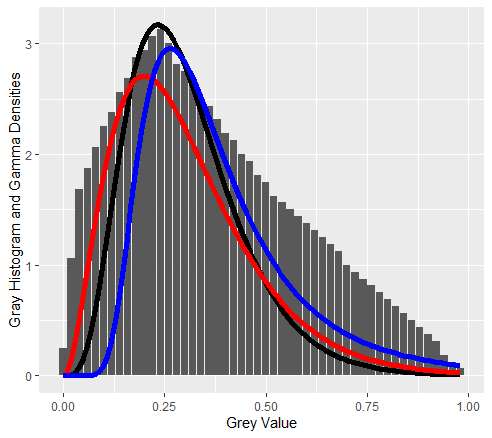
\includegraphics[width=4in]{homework/picture/urban.png} 
    	\caption{Curve fitting distribution}
    \end{figure}

	\begin{figure}[h] % [h] forces the figure to be output where it is defined in the code (it suppresses floating)
		\centering
		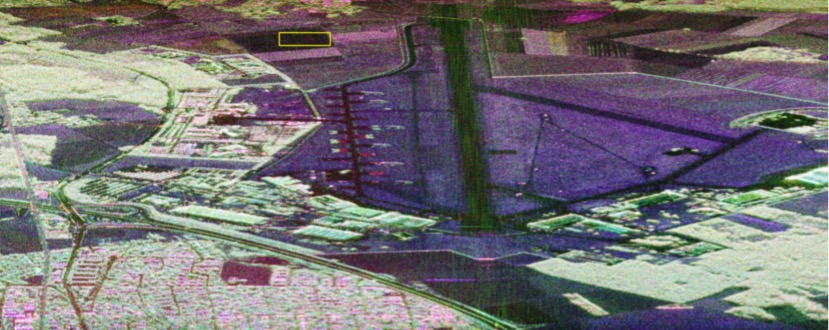
\includegraphics[width=4in]{homework/picture/ori.png} %Example image
		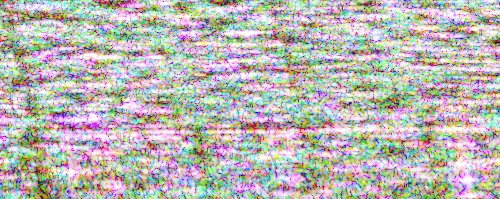
\includegraphics[width=2in]{homework/picture/pic.jpg}
		\caption{Original image(left) and Captured image(right)}
	\end{figure}

\end{document}
